This section discusses the various details about software implemented in detail.

\section{Design}

The software is implemented in Java using ArangoDB as backend database. The application has 3 layer structure as per Figure \ref{fig:appdesign}. The database layer which is the ArangoDB database itself. The business layer, this layer contains all the logic for talking to the backend ArangoDB, the clustering algorithms and other functions. The application has 2 frontend: Web application which is made using the Spring framework in Java and a simple command line application. Both the front end uses the same business layer hence providing same functionality. 

The way this project was strategised was to make command line first for easy testing of the core functionality like clustering, inserting the data, getting the data etc. Then the same core libraries are called via the web application. Web application was created for ease of use and multiple simultaneous analysis. Another reason for keeping the command line application was, some of the commands took too long to process. The connection between the server and the client used to timeout. Websocket's helped keeping the connection alive but once the connection is broken the results were lost in the process.

The whole project has 3 modules namely core, cmdapp, webapp. Gradle build tool was used for compiling, testing and running the application. 

\begin{figure}[ht]
	\centering
	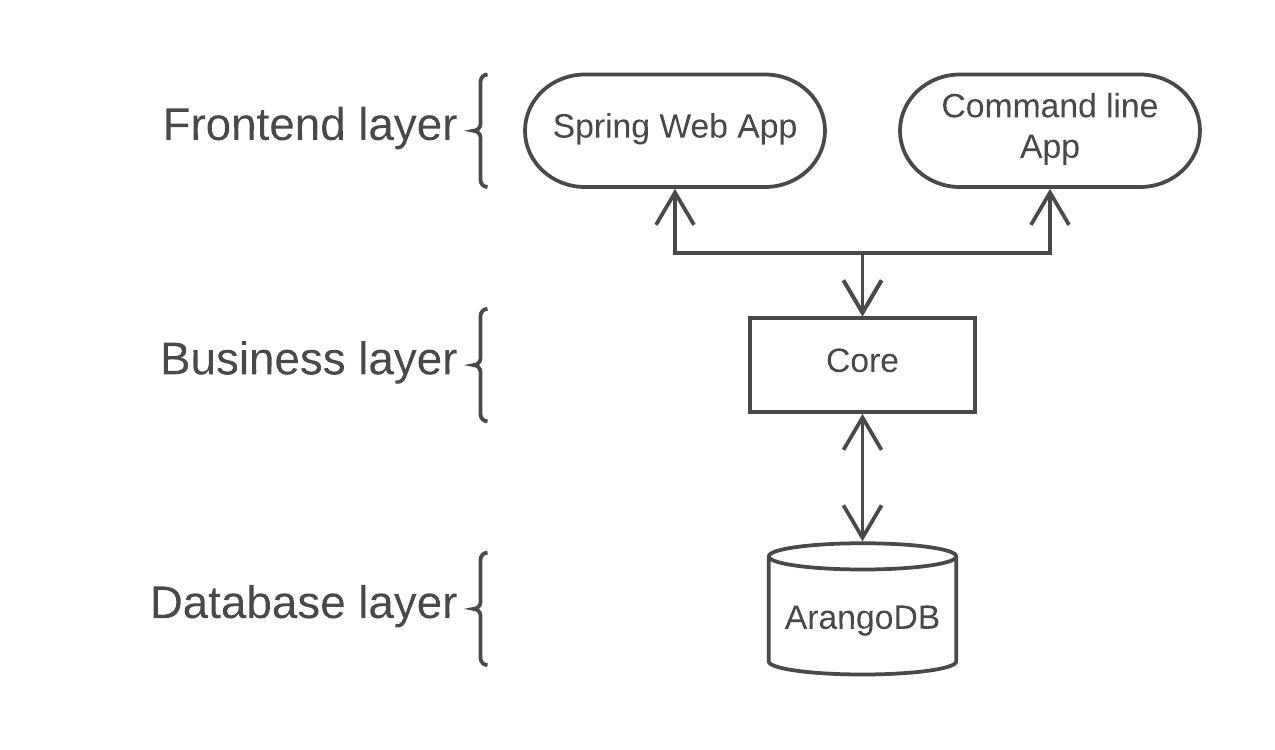
\includegraphics[width=300pt]{appdesign}
	\caption{\label{fig:appdesign} Structure of the app}
\end{figure}

\subsection{ArangoDB}

ArangoDB is a multi-model database. It supports three data models namely key/value, documents, graphs and a unified query language called AQL. AQL is very similar to SQL query language. AQL is used for CRUD operations. It provides scalabe and highly efficient queries. It uses JSON as a default storage schema. 

The application uses this database for all the heavy duty data operations like grouping, summing, filtering neighbours etc. The reason a database was used instead of doing it directly in Java was for faster development, thread-safety and also the indexes provided by the database for faster queries. 

\subsection{Core}

This business layer of the application contains all the core logic. It contains all the query, the driver to talk to ArangoDB, the logic for converting from and to csv etc. The core module uses spring-context which is an application IoC (Inversion of Control) container. This container can be consumed by any application by adding the library and providing the database connection configuration. This saves the other application from creating each and every object. The IoC container creates the object for the application automatically at runtime. The strategy was to create a library which contains all main logic and which can be consumed by any kind of application. This can be seen as we have implemented in two applications command line and web application.

Apart from using IoC containers, the main design pattern used by this module of application is the Command Pattern\cite{dupire2001command}. In this pattern, an object is encapsulated with all the information needed to perform an action. The biggest feature of the command pattern is that it can be executed at any point in time. The command in our case is executed by a Command executor. This separation of the actual command and executor allows for greater changes in the future of the project. It provides a lot of flexibility and ease of adding and replacing commands in later stages of the development. One of the purposes of using command pattern was the certain routines in the application are quite slow e.g. distance based clustering. The command pattern creates a unified way for getting the updates/progress of a task being executed.

The drawbacks of this pattern is it makes the source code larger quickly because one file can only represent one command. The number of files in the project increases very quickly. Command names are usually big and so goes for the file names. The order of commands becomes important at later stages and can jeopardize the reliability of the system\cite{dupire2001command}.

\begin{figure}[!ht]
	\centering
	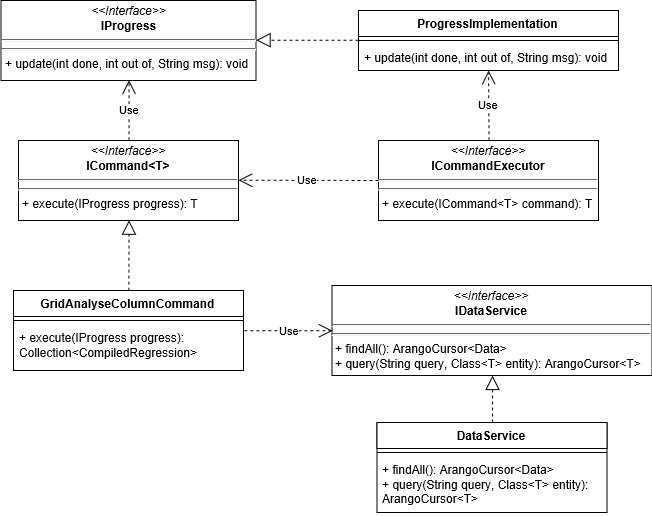
\includegraphics[width=300pt]{umlcore}
	\caption{\label{fig:umlcore} UML diagram of the command pattern in the core module}
\end{figure}

Figure\ref{fig:umlcore}, shows the implementation of command pattern. Only one Concrete command (GridAnalyseColumnCommand) is been shown. There are various commands implemented for data insertion, data deletion, distance based analysing etc. It can be seen from the figure\ref{fig:umlcore} that no implementation is defined for ICommandExecutor. This is because the modules consuming this core module library can implement according to their need. Similarly for the IProgress, modules can implement their own version depending on their type of the application. The parameters of the command are supplied when creating the instance of the object. The command object constructor contains all the necessary arguments needs for execution at later stage.

\subsection{Webapp}

The web application is built on Spring framework. It comes with IoC container which can easily pass in the database connection to the core library being consumed. In this module, the progress and command executor interfaces are implements to the needs of the web application. The progress interface implementation uses WebSocket for sending the update of how much work has been completed by the command. WebSocket is  full-duplex communication channel over TCP which allows server and client to send messages to each other asynchronously.

The application maps the REST APIs to the Commands in the core module. The UI of the web application uses AngularJS which is a client side front end web framework. AngularJS framework allows to makes calls to the REST Endpoints and also act accordingly to the messages received by the server through WebSocket.

\subsection{Command Line}

The command line application also uses the core module to do similar task. The mapping is from command line arguments to core module's command. In this module, as well a different implementation is done for the progress and command executor interfaces as this time the diplay and execution is in commandline. Since the core module uses IoC container. Spring-context was added and application context was created at the start of the applicaton. The arguments were parsed via the JCommander library. 

\section{Results and Optimizations}

\section{Existence of functional relation}

